\chapter{Large Language Models}
Quando si parla di Large Language Models (LLM) \cite{minaee2024largelanguagemodelssurvey}, si fa riferimento a modelli di deep learning, quindi basati su reti neurali profonde, progettati per elaborare dati non strutturati, in particolare il testo, in linguaggio naturale. Questi modelli, addestrati su enormi quantità di dati testuali, sono in grado di comprendere il contesto ricevuto, generare testi coerenti e rispondere a input linguistici in modo accurato. Alcuni modelli avanzati sono anche in grado di gestire contenuti multimediali, come audio, immagini e video, attraverso estensioni multimodali, sebbene la loro competenza primaria riguardi la comprensione e generazione del linguaggio naturale.

\section{Le origini}
Analizziamo prima le origini degli LLM e i principali sviluppi che hanno portato alla creazione di modelli sempre più avanzati e performanti.

\subsection{Modelli di linguaggio tradizionali}
Prima dell'introduzione delle reti neurali, i modelli di linguaggio si basavano principalmente su approcci statistici. Questi metodi erano utili per stimare la probabilità di una parola in una sequenza, ma avevano limitazioni significative nella capacità di catturare le dipendenze a lungo raggio e le complessità semantiche e sintattiche del linguaggio naturale.
\begin{itemize}
	\item \textbf{Modelli N-gramma}: Questi modelli stimano la probabilità di una parola in base alle \(N - 1\) parole precedenti. Ad esempio, un modello bigramma (\(N = 2\)) calcola la probabilità di una parola basandosi solo sulla parola immediatamente precedente, mentre uno trigramma (\(N = 3\)) considera le due parole precedenti. Gli N-grammi sono stati ampiamente utilizzati per la traduzione automatica e il riconoscimento del parlato, ma soffrono di alcuni problemi:
	\begin{itemize}
		\item \textbf{Sparsità dei dati}: Più aumenta il valore di \(N\), più diventa difficile raccogliere abbastanza dati per coprire tutte le possibili sequenze di \(N\) parole. Questo porta a un problema di sparsità, dove molte combinazioni di parole non sono mai state osservate durante l'addestramento.
		\item \textbf{Dipendenze a lungo raggio}: Gli N-grammi non possono catturare relazioni a lungo raggio tra le parole. Ad esempio, in una frase complessa, parole che appaiono molto distanti possono essere fortemente correlate, ma un modello N-gramma con un \(N\) basso non sarà in grado di cogliere questa relazione.
	\end{itemize}
	\item \textbf{Modelli a Catena di Markov}: I modelli di Markov, come gli N-grammi, ipotizzano che la probabilità di utilizzo di una parola dipenda solo da un numero limitato di parole precedenti. Nelle catene di Markov di ordine \(k\), la probabilità di una parola viene calcolata in base alle \(k\) parole precedenti. Questi modelli sono molto simili agli N-gramma e condividono molte delle stesse limitazioni. Una variante di questi modelli, le Hidden Markov Models (HMM) \cite{stolcke1994bestfirstmodelmerginghidden}, sono state ampiamente utilizzate per compiti come il riconoscimento del parlato e il part-of-speech tagging, dove lo stato latente rappresenta informazioni nascoste (ad esempio, la parte del discorso) che generano l'output osservato (la parola).
	\item \textbf{Modelli di Massima Entropia (MaxEnt)}: Questi modelli fanno uso di informazioni contestuali multiple (feature) per stimare la probabilità di una parola, massimizzando l'entropia soggetta a vincoli. I modelli di massima entropia non fanno assunzioni forti sul contesto e possono combinare diverse fonti di informazione per fare previsioni, ma anch'essi sono limitati quando si tratta di catturare relazioni a lungo termine nel testo.
	\item \textbf{Modelli di Interpolazione e Smoothing}: Per mitigare il problema della sparsità nei modelli N-gramma, vennero introdotte tecniche di smoothing come Laplace smoothing o Kneser-Ney smoothing, che assegnano probabilità non nulle anche a sequenze di parole mai osservate. Anche tecniche di interpolazione sono state sviluppate per combinare modelli N-gramma di diversi ordini, migliorando così la robustezza.
\end{itemize}
Questi modelli, pur essendo stati pionieristici e molto utilizzati, avevano una comprensione limitata del linguaggio. Erano rigidi nella loro capacità di generalizzare, poiché dipendevano da pattern ripetitivi che non potevano adattarsi facilmente a frasi complesse o nuove combinazioni di parole. Questo ha spianato la strada all'introduzione di approcci più avanzati, come le reti neurali ricorrenti (RNN), che potevano superare queste limitazioni catturando relazioni più complesse tra le parole e gestendo dipendenze a lungo raggio.

\subsection{Recurrent Neural Networks}
Negli anni '90 e 2000, l'avvento delle Recurrent Neural Networks (RNN) ha segnato un importante passo avanti nel campo del Natural Language Processing. A differenza dei modelli tradizionali, le RNN sono state progettate per gestire dati sequenziali, permettendo alla rete di avere una memoria interna che si aggiorna ad ogni passo temporale. Questa capacità di elaborare input di lunghezza variabile ha reso le RNN particolarmente adatte per attività come la traduzione automatica, il riconoscimento del parlato e la generazione di testo, dove il contesto a lungo termine gioca un ruolo cruciale.
Le RNN, in teoria, possono modellare le dipendenze temporali tra elementi in una sequenza, poiché ogni neurone dell'RNN riceve non solo l'input corrente ma anche l'output del passo precedente. Questo crea un meccanismo di feedback che consente alla rete di "ricordare" informazioni di stati passati e di propagare queste informazioni attraverso la rete per più passaggi temporali.

\subsubsection{Architettura delle RNN}
La struttura base di una RNN consiste in una serie di layer ricorrenti che prendono in input una sequenza temporale di dati e calcolano uno stato nascosto ad ogni passo temporale. Questo stato nascosto viene poi utilizzato come input per il passo successivo, insieme al nuovo dato della sequenza. La ricorrenza nella rete permette di mantenere una "memoria" delle informazioni passate, e tale informazione può essere utilizzata per prendere decisioni basate sul contesto storico del testo. Nelle applicazioni NLP, questo significa che ogni parola nella sequenza può influenzare le previsioni delle parole successive.

\subsubsection{Problema del Vanishing Gradient}
Per quanto le RNN abbiano portato una grande innovazione, questi modelli soffrivano di un problema noto come Vanishing Gradient. Questo fenomeno si verifica durante la fase di addestramento, quando si utilizzano tecniche di ottimizzazione basate su gradienti, come la Backpropagation Through Time (BPTT). Con l'aumentare della lunghezza delle sequenze, i gradienti calcolati per aggiornare i pesi della rete tendevano a diminuire esponenzialmente, rendendo difficile l'aggiornamento dei parametri dei layer ricorrenti. Di conseguenza, le RNN faticavano ad apprendere dipendenze a lungo termine tra parole o frasi distanti all'interno di un testo, limitando la loro capacità di comprendere il contesto globale in una sequenza lunga.

\subsubsection{Problema dell'Exploding Gradient}
In contrasto con il problema del vanishing gradient, a volte si osservava anche un fenomeno opposto noto come Exploding Gradient, in cui i gradienti crescevano esponenzialmente durante l'addestramento, causando instabilità nei processi di ottimizzazione. Questo fenomeno richiedeva l'uso di tecniche di regolazione, come il Gradient Clipping, per evitare che i gradienti esplodessero durante la retropropagazione.

\subsubsection{Applicazioni delle RNN}
Nonostante questi problemi, le RNN sono state adottate con successo in vari campi del NLP. Esse erano particolarmente adatte per applicazioni come:
\begin{itemize}
	\item \textbf{Traduzione automatica}: Dove la sequenza di parole in una lingua veniva mappata in una sequenza di parole in un'altra lingua.
	\item \textbf{Riconoscimento del parlato}: Si riconoscono parole e frasi a partire da segnali audio, grazie alla capacità delle reti di modellare le dipendenze temporali nei dati acustici.
	\item \textbf{Generazione di testo}: Le RNN potevano generare sequenze di testo una parola alla volta, tenendo conto del contesto delle parole precedenti.
\end{itemize}

\subsection{Gated Recurrent Neural Networks}
Una delle principali limitazioni delle Recurrent Neural Networks (RNN) tradizionali, ovvero la difficoltà nel catturare le dipendenze a lungo termine, è stata mitigata con l'introduzione delle Gated Recurrent Neural Networks (GRNN). Questi modelli rappresentano una famiglia di RNN che integrano meccanismi di gating, i quali, permettono alla rete di controllare in modo più efficiente il flusso delle informazioni, consentendo così alla stessa di decidere quali informazioni mantenere, aggiornare o dimenticare nel corso dell'elaborazione di una sequenza. Questo approccio consente di gestire con maggiore efficacia i problemi associati al vanishing gradient e all'incapacità di modellare sequenze lunghe.
Le due implementazioni più popolari di Gated RNN sono le Long Short-Term Memory (LSTM) e le Gated Recurrent Units (GRU), che hanno dimostrato una straordinaria efficacia in molte applicazioni di NLP e apprendimento sequenziale.

\subsubsection{Long Short-Term Memory (LSTM)}
Le Long Short-Term Memory \cite{10.1162/neco.1997.9.8.1735,sak2014longshorttermmemorybased,cheng2016longshorttermmemorynetworksmachine}, proposte da Hochreiter e Schmidhuber nel 1997, sono state progettate appositamente per affrontare le limitazioni delle RNN classiche. Esse sono costituite da una struttura più complessa rispetto alle RNN standard, con l'inclusione di una cella di memoria interna e tre principali gate (o porte), che regolano il flusso delle informazioni all'interno della rete. Questi gate consentono alla rete di conservare informazioni per periodi di tempo più lunghi e di decidere quali dati devono essere eliminati, quali devono essere aggiornati e quali devono essere trasmessi all'output. Essi sono:
\begin{itemize}
	\item \textbf{Input Gate}: Questo gate decide quali nuove informazioni devono essere aggiunte alla cella di memoria. L'input gate prende in input il nuovo dato e lo combina con lo stato precedente della cella di memoria, determinando quali informazioni aggiornare.
	\item \textbf{Forget Gate}: È il gate che controlla quali informazioni della cella di memoria devono essere eliminate o mantenute. Il forget gate è essenziale per evitare che la cella di memoria si riempia di informazioni obsolete o irrilevanti, permettendo alla rete di "dimenticare" informazioni non necessarie.
	\item \textbf{Output Gate}: Il gate di output stabilisce quale parte della cella di memoria deve essere utilizzata per generare l'output corrente. Questo processo è cruciale per garantire che l'output sia basato non solo sull'input attuale, ma anche su un contesto ben regolato dalle informazioni memorizzate in precedenza.
\end{itemize}
L'aggiunta di questi gate permette alle LSTM di catturare dipendenze a lungo termine all'interno di sequenze, risolvendo il problema delle sequenze estese e migliorando significativamente le prestazioni in compiti come la traduzione automatica, il riconoscimento del parlato e la generazione di testo.

\paragraph{Vantaggi delle LSTM}
Sono particolarmente potenti quando si tratta di modellare sequenze lunghe e complesse. La loro capacità di mantenere una memoria controllata, attraverso i gate, permette di evitare la perdita di informazioni critiche durante l'elaborazione delle sequenze, il che le rende adatte per:
\begin{itemize}
	\item \textbf{Predizione di serie temporali}: dove la rete deve tenere conto di eventi molto distanti nel tempo.
	\item \textbf{Traduzione automatica}: in cui la comprensione di frasi complete dipende dalle informazioni precedenti nel testo.
	\item \textbf{Sentiment Analysis}: dove è essenziale catturare il contesto globale di un paragrafo per comprendere il tono emotivo.
\end{itemize}
Nonostante la loro efficacia, le LSTM possono essere computazionalmente costose, soprattutto su sequenze molto lunghe o dataset di grandi dimensioni, data la complessità dell'architettura.

\subsubsection{Gated Recurrent Unit (GRU)}
Le Gated Recurrent Units, introdotte da Cho et al. nel 2014 \cite{chung2014empiricalevaluationgatedrecurrent}, sono una variante semplificata delle LSTM, progettata per mantenere le stesse capacità di modellazione delle dipendenze a lungo termine, ma con un'architettura più leggera e meno computazionalmente intensa. Le GRU combinano alcune delle funzioni dei gate delle LSTM in modo da ridurre il numero di operazioni per passo temporale, semplificando così il processo di apprendimento.
Esse contengono solo due gate principali:
\begin{itemize}
	\item \textbf{Reset Gate}: Esso è il gate che controlla il modo in cui il nuovo input viene combinato con la memoria precedente. Se il reset gate è attivo, il modello può "ripartire" con un nuovo stato, dimenticando parte o tutte le informazioni precedenti.
	\item \textbf{Update Gate}: Si tratta del gate che decide quanto della memoria precedente deve essere mantenuto e quanto deve essere aggiornato con nuove informazioni. L'update gate combina le funzioni di input e forget gate delle LSTM in un unico meccanismo, permettendo alla GRU di essere più efficiente.
\end{itemize}

\paragraph{Vantaggi delle GRU} Hanno guadagnato popolarità perché, pur offrendo prestazioni simili alle LSTM, tendono a essere più efficienti dal punto di vista computazionale. Poiché hanno meno parametri, risultano spesso più veloci da addestrare e meno suscettibili al problema del sovradimensionamento (\textit{overfitting}), specialmente quando il dataset di addestramento non è troppo ampio. Questo le rende una scelta ideale per:
\begin{itemize}
	\item \textbf{Sistemi in tempo reale}: dove la velocità di calcolo è cruciale.
	\item \textbf{Applicazioni su dispositivi con risorse limitate}: come gli smartphone o dispositivi IoT.
\end{itemize}
In molti scenari pratici, le GRU e le LSTM ottengono risultati comparabili. Tuttavia, la scelta tra le due dipende spesso dalle esigenze specifiche dell'applicazione: le LSTM possono essere preferibili per problemi che richiedono una memoria più complessa, mentre le GRU risultano più efficienti quando è importante bilanciare prestazioni e velocità.

\section{Transformer}
Il modello Transformer, introdotto nel 2017 nel paper "Attention is All You Need" di Vaswani et al. \cite{vaswani2023attentionneed}, ha rivoluzionato il campo dell'elaborazione del linguaggio naturale (NLP) e molti altri ambiti del deep learning. Rispetto ai modelli precedenti, il Transformer ha offerto vantaggi significativi in termini di velocità, scalabilità e accuratezza nei compiti sequenziali.

Sviluppato da ricercatori di Google Brain e Google Research, il Transformer adotta un'architettura di tipo encoder-decoder e sfrutta i meccanismi di attention per catturare relazioni tra le parole all'interno di una sequenza. Questo approccio si è dimostrato più efficace rispetto alle reti neurali ricorrenti, poiché consente di gestire le dipendenze a lungo termine in modo più efficiente e di elaborare sequenze di lunghezza variabile senza le limitazioni delle unità ricorrenti e dei modelli tradizionali.

Uno dei principali vantaggi del Transformer è la sua natura altamente parallelizzabile, che deriva dall'assenza di unità ricorrenti. Questo lo rende più facile da addestrare su hardware accelerato, come GPU e TPU, permettendo di scalare i modelli a dimensioni mai viste prima \cite{10.1145/3442188.3445922}. In più permette anche di gestire sequenze di token più lunghe \cite{ding2023longnetscalingtransformers1000000000}.

Originariamente concepito per migliorare le architetture esistenti nei task di traduzione automatica \cite{wu2016googlesneuralmachinetranslation,luong2015effectiveapproachesattentionbasedneural,bahdanau2016neuralmachinetranslationjointly}, il Transformer si è rivelato estremamente versatile. Da allora, è stato adattato con successo a una vasta gamma di applicazioni, tra cui il NLP, la computer vision (ad esempio, con i Vision Transformer, ViT) \cite{Khan_2022}, il Reinforcement Learning \cite{zheng2023secretsrlhflargelanguage} (ad esempio con il Decision Transformer) \cite{chen2021decisiontransformerreinforcementlearning}, i Large Action Models (LAM), il riconoscimento vocale (attraverso il modello Conformer \cite{gulati2020conformerconvolutionaugmentedtransformerspeech} oppure con Whisper \cite{radford2022robustspeechrecognitionlargescale}), applicazioni multimodali di vario tipo (modello Perceiver \cite{jaegle2021perceivergeneralperceptioniterative,jaegle2022perceiveriogeneralarchitecture}), ad esempio per la generazione di immagini e video \cite{esser2024scalingrectifiedflowtransformers}, e persino software strategici \cite{ruoss2024grandmasterlevelchesssearch}. La sua versatilità continua a spingersi in nuovi ambiti di ricerca \cite{transformersstateofarthuggingface,choromanski2022rethinkingattentionperformers}.

\subsection{Architettura del Transformer}
I migliori modelli di trasduzione sequenziali precedenti erano basati su complesse strutture ricorrenti, che includevano un encoder e un decoder \cite{cho2014learningphraserepresentationsusing,sutskever2014sequencesequencelearningneural}. I più avanzati tra questi integravano anche un meccanismo di attenzione \cite{vaswani2023attentionneed}. Il Transformer, al contrario, ha abbandonato le strutture ricorrenti in favore di un'architettura interamente basata sui meccanismi di attention, pur mantenendo la struttura encoder-decoder \cite{illustratedtransformer}.
\begin{figure}[!t]
	\centering
	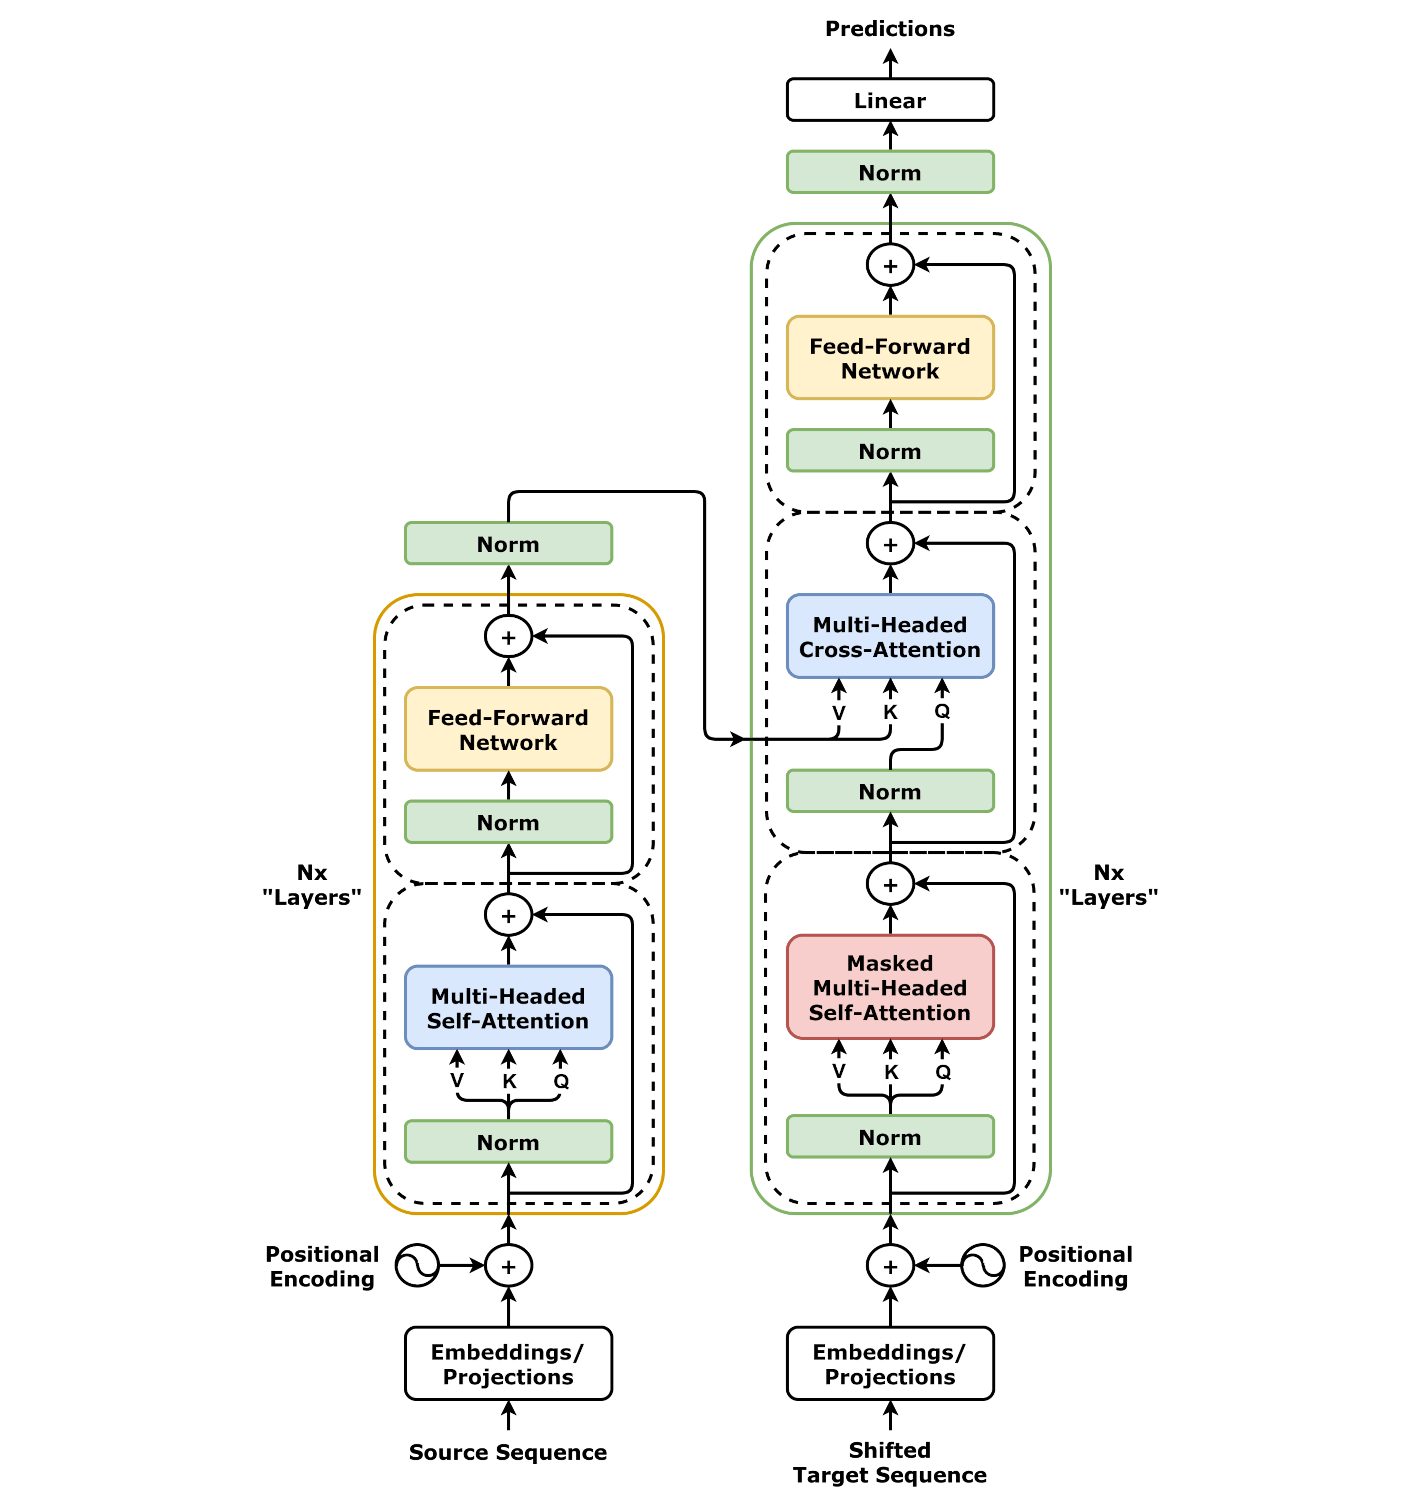
\includegraphics[width=1.05\linewidth]{Images/cap1/Transformer,_full_architecture.png}
	\caption{Transformer: a sinistra l'encoder, a destra il decoder \cite{transformervisuals}.}
	\label{fig:transformer}
\end{figure}

Nonostante esistano diverse varianti del Transformer, tutte condividono le seguenti componenti principali e sequenza di operazioni \cite{phuong2022formalalgorithmstransformers}:
\begin{itemize}
	\item \textbf{Tokenizer}: Converte il testo in input in una sequenza di token, che rappresentano le unità di base elaborate dal modello.
	\item \textbf{Embedding Layer}: Mappa i token in vettori di embedding, i quali catturano le relazioni semantiche tra le parole, includendo informazioni sia sul significato che sulla posizione dei token nella sequenza.
	\item \textbf{Transformer Layer}: Costituiscono il cuore del modello. Ogni Transformer layer estrae informazioni sempre più complesse attraverso più livelli. Questi strati multilivello comprendono sia l'encoder che il decoder (nella versione standard del Transformer).
	\item \textbf{Un-embedding Layer}: Converte le rappresentazioni vettoriali finali in una distribuzione di probabilità sui token del vocabolario, permettendo così di generare il testo in output.
\end{itemize}
Le componenti verranno ora esaminate nel dettaglio:

\subsubsection{Tokenizer}
Il Transformer non può processare nativamente dati di tipo testuale, si occupa invece di analizzare sequenze numeriche. Per questo motivo è necessario convertire il testo in input in qualche modo, il primo passo consiste nell'associare un intero per ogni carattere o comunque per una piccola sequenza di caratteri (token). Il set di tutti i token generati viene chiamato vocabolario.

\subsubsection{Embedding Layer}
Ogni token viene convertito in un vettore di embedding \cite{mikolov2013distributedrepresentationswordsphrases}, e la corrispondenza tra il token e il suo vettore viene salvata in una \textit{"lookup table"}. La dimensione di questi vettori di embedding, nota anche come hidden dimension \cite{gpt2backbone} o embedding size \cite{devlin2019bertpretrainingdeepbidirectional}, varia in base all'implementazione utilizzata. Nel paper originale viene indicata con $d_{\text{model}} = 512$ \cite{vaswani2023attentionneed}, ma esistono modelli con dimensioni differenti, come ad esempio GPT-2 con $d_{\text{model}} = 768$ \cite{gpt2backbone}, BERT con $d_{\text{model}} = 768$ \cite{devlin2019bertpretrainingdeepbidirectional}, o T5 con $d_{\text{model}} = 1024$ \cite{raffel2023exploringlimitstransferlearning}.

Grazie a questa conversione, il Transformer è in grado di interpretare il testo in modo più strutturato, ma emergono alcune limitazioni. In particolare, parole diverse con significato simile (sinonimia) possono produrre embedding differenti, mentre parole con più significati (polisemia) tendono a generare lo stesso embedding indipendentemente dal contesto. Questo porta spesso a rappresentazioni ambigue e potenzialmente errate.
Per ovviare a queste limitazioni, si possono usare modelli di embedding pre-addestrati come Word2Vec \cite{mikolov2013efficientestimationwordrepresentations}, sviluppato da un team di Google guidato da Tomas Mikolov nel 2013, o GloVe \cite{pennington-etal-2014-glove}, sviluppato dalla Stanford University. Entrambi gli approcci catturano relazioni semantiche tra le parole grazie a tecniche basate su co-occorrenza e distribuzione dei termini.
In alternativa, è possibile addestrare un modello di embedding specifico per il task, per ottenere rappresentazioni più precise nel contesto d'uso. Una delle soluzioni avanzate a questo problema è l'uso di modelli che supportano i multi-sense embeddings \cite{camachocollados2018wordsenseembeddingssurvey,reisinger-mooney-2010-multi}, i quali assegnano rappresentazioni vettoriali diverse a parole con significati differenti a seconda del contesto in cui appaiono, migliorando così la gestione di sinonimia e polisemia.

\subsubsection{Transformer Layer}
\textit{Vedi Paragrafo} \ref{sec:transformer-layer} \textit{per una trattazione completa.}

\subsubsection{Un-embedding Layer}
A seguito dell'elaborazione dell'input, il vettore di output viene convertito in una distribuzione di probabilità sui token del vocabolario. Questo processo è noto come \textit{"un-embedding"} e viene realizzato attraverso un layer di output softmax, che restituisce la probabilità di ciascun token in base al contesto.
\begin{align}
	\text{UnEmbed}(x) = \text{softmax}(xW + b)
\end{align}
Il token con la probabilità più alta viene selezionato come output finale.

\subsection{Transformer Layer}
\label{sec:transformer-layer}
I modelli Transformer sono costituiti da più strati di Transformer Layer, ognuno dei quali può assumere configurazioni differenti a seconda dell'implementazione e dell'utilizzo specifico che verrà fatto. In particolare, si farà riferimento alla versione originale proposta da Vaswani et al. \cite{vaswani2023attentionneed}, che comprende sia un encoder che un decoder.
\begin{figure}[!t]
	\centering
	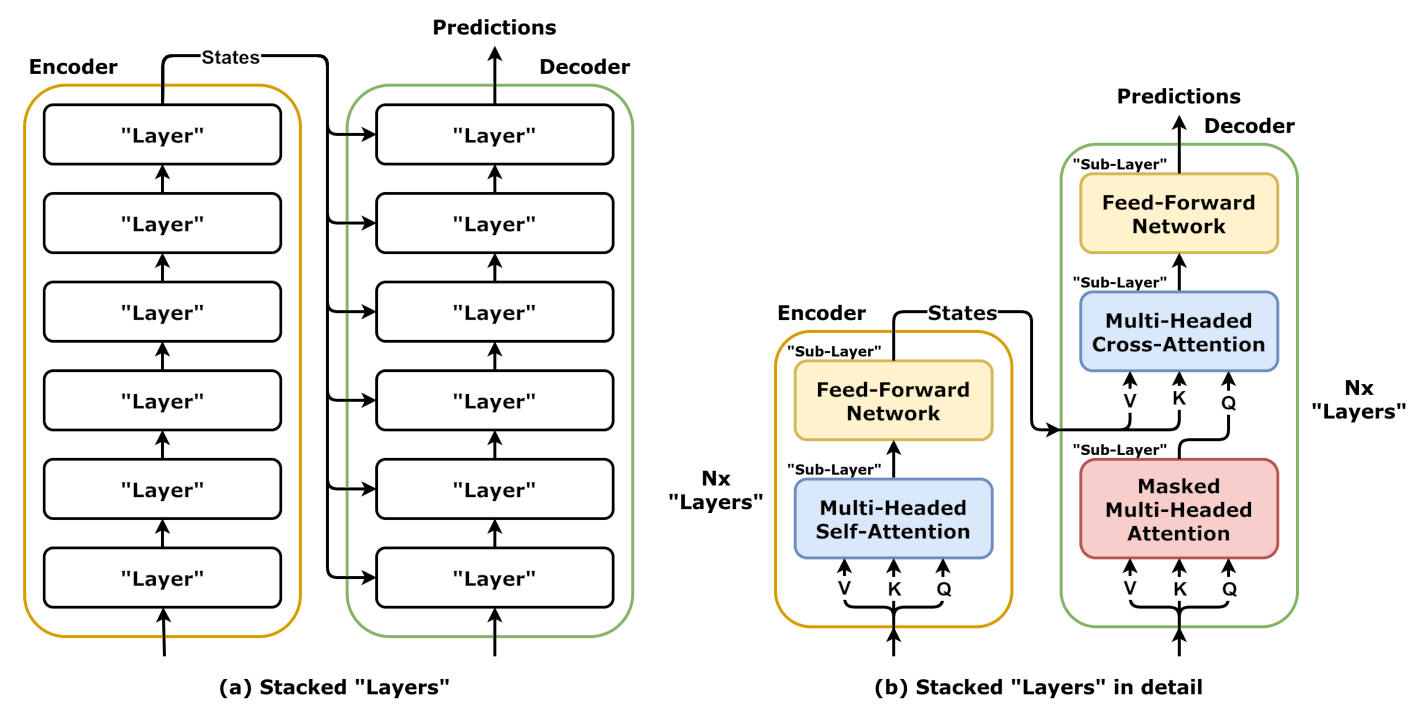
\includegraphics[width=\linewidth]{Images/cap1/Transformer,_stacked_layers_and_sublayers.png}
	\caption{Architettura a strati del Transformer.}
	\label{fig:transformer-sublayers}
\end{figure}
Il numero di layer, la dimensione dei vettori di embedding e la dimensione dei feed-forward neural network sono iperparametri che possono essere regolati per adattare la rete neurale a diversi compiti e dataset.
In generale, un numero maggiore di layer permette al Transformer di catturare relazioni più complesse e di apprendere rappresentazioni più dettagliate, ma richiede anche più risorse computazionali e tempo di addestramento.
A seguire le caratteristiche implementative del Transformer Layer presentato nel paper originale.

\subsubsection{Encoder}
L'encoder è costituito da una pila di \(N\) layer identici (6 nell'originale di Vaswani et al.) \cite{vaswani2023attentionneed}, ciascuno dei quali opera in parallelo sugli input. Ogni layer è composto da due sub-layer principali:
\begin{itemize}
	\item \textbf{Multi-Headed Self-Attention}: Questo meccanismo consente ad esso di catturare le relazioni tra le parole all'interno della stessa sequenza. Ogni parola può "attenzionare" tutte le altre parole della sequenza, calcolando un peso relativo in base alla loro rilevanza nel contesto. Grazie a diverse "teste" di attenzione, il modello può osservare la sequenza da prospettive diverse, cogliendo dipendenze sia a breve che a lungo termine. Questo è fondamentale per comprendere le relazioni semantiche complesse all'interno di una frase e per gestire le dipendenze a lungo raggio.
	\item \textbf{Feed-Forward Neural Network}: Dopo la fase di attenzione, ogni vettore di embedding viene elaborato da uno o più layer feed-forward. Questa rete opera in parallelo su tutti i token della sequenza, applicando una trasformazione non lineare che permette al modello di arricchire le rappresentazioni dei token e di catturare pattern più complessi. La rete feed-forward è costituita da due layer densi con una funzione di attivazione intermedia, generalmente una ReLU (Rectified Linear Unit), per introdurre non linearità nell'elaborazione. In certi casi, si possono utilizzare funzioni di attivazione diverse, come la GELU (Gaussian Error Linear Unit), che ha dimostrato di migliorare le prestazioni in alcuni compiti \cite{hendrycks2023gaussianerrorlinearunits}.
\end{itemize}
Entrambi i sub-layer sono seguiti da una Residual Connection e da un Layer Normalization \cite{ba2016layernormalization}. Le Residual Connections permettono di "saltare" i sub-layer e aggiungono l'input originale direttamente all'output del sub-layer stesso, facilitando il flusso del gradiente attraverso i layer. Questo accorgimento aiuta a prevenire il problema del vanishing gradient, che ostacolerebbe l'apprendimento nei modelli profondi. Inoltre, esse ne accelerano il processo, poiché mantengono in circolazione informazioni non modificate, mentre la rete si concentra sulla modellazione di pattern più complessi.
Il Layer Normalization, applicato dopo ogni Residual Connection, stabilizza l'addestramento mantenendo il range delle attivazioni all'interno di una scala gestibile. Questo aiuta il modello a convergere più rapidamente durante il processo di ottimizzazione, riducendo l'instabilità causata dalle variazioni nei valori delle attivazioni. Esistono diverse alternative al Layer Normalization come il Root Mean Square Layer Normalization (RMS-LN) \cite{zhang2019rootmeansquarelayer}, il BatchNorm usato nei modelli della famiglia Llama, o altri \cite{https://doi.org/10.5281/zenodo.3525484}.

\paragraph{Noam Learning Rate Scheduler}
Un'altra strategia utilizzata per stabilizzare l'addestramento è l'impiego di un meccanismo di warmup del learning rate, implementato tramite il cosiddetto Noam Learning Rate Scheduler \cite{noamlearningrate,vaswani2023attentionneed}. Questo scheduler aumenta gradualmente il learning rate nei primi \(w\) step dell'addestramento (warmup steps), per poi ridurlo in proporzione inversa alla radice quadrata del numero \(t\) di passi temporali.
\begin{align}
	\text{learning rate} = \alpha \frac{1}{\sqrt{d_{\text{model}}}} \min \left(\frac{1}{\sqrt{t}}, \frac{t}{w^{3/2}} \right)
	\label{eq:noam-scheduler}
\end{align}
Tale schema evita oscillazioni improvvise nel processo di ottimizzazione e garantisce una fase iniziale di esplorazione dello spazio delle soluzioni, migliorando la stabilità complessiva della rete.

Tuttavia, ricerche successive hanno dimostrato che il meccanismo di warmup non è sempre strettamente necessario, poiché, applicando la normalizzazione prima della multi-head attention, piuttosto che dopo, si può ridurre o eliminare la necessità del warmup, stabilizzando comunque l'apprendimento e velocizzando la convergenza \cite{xiong2020layernormalizationtransformerarchitecture} (vedi \figurename{~\ref{fig:encoder}}).
\begin{figure}[!t]
    \centering
    \begin{minipage}{0.48\textwidth}
        \centering
		\hspace*{-2cm}
        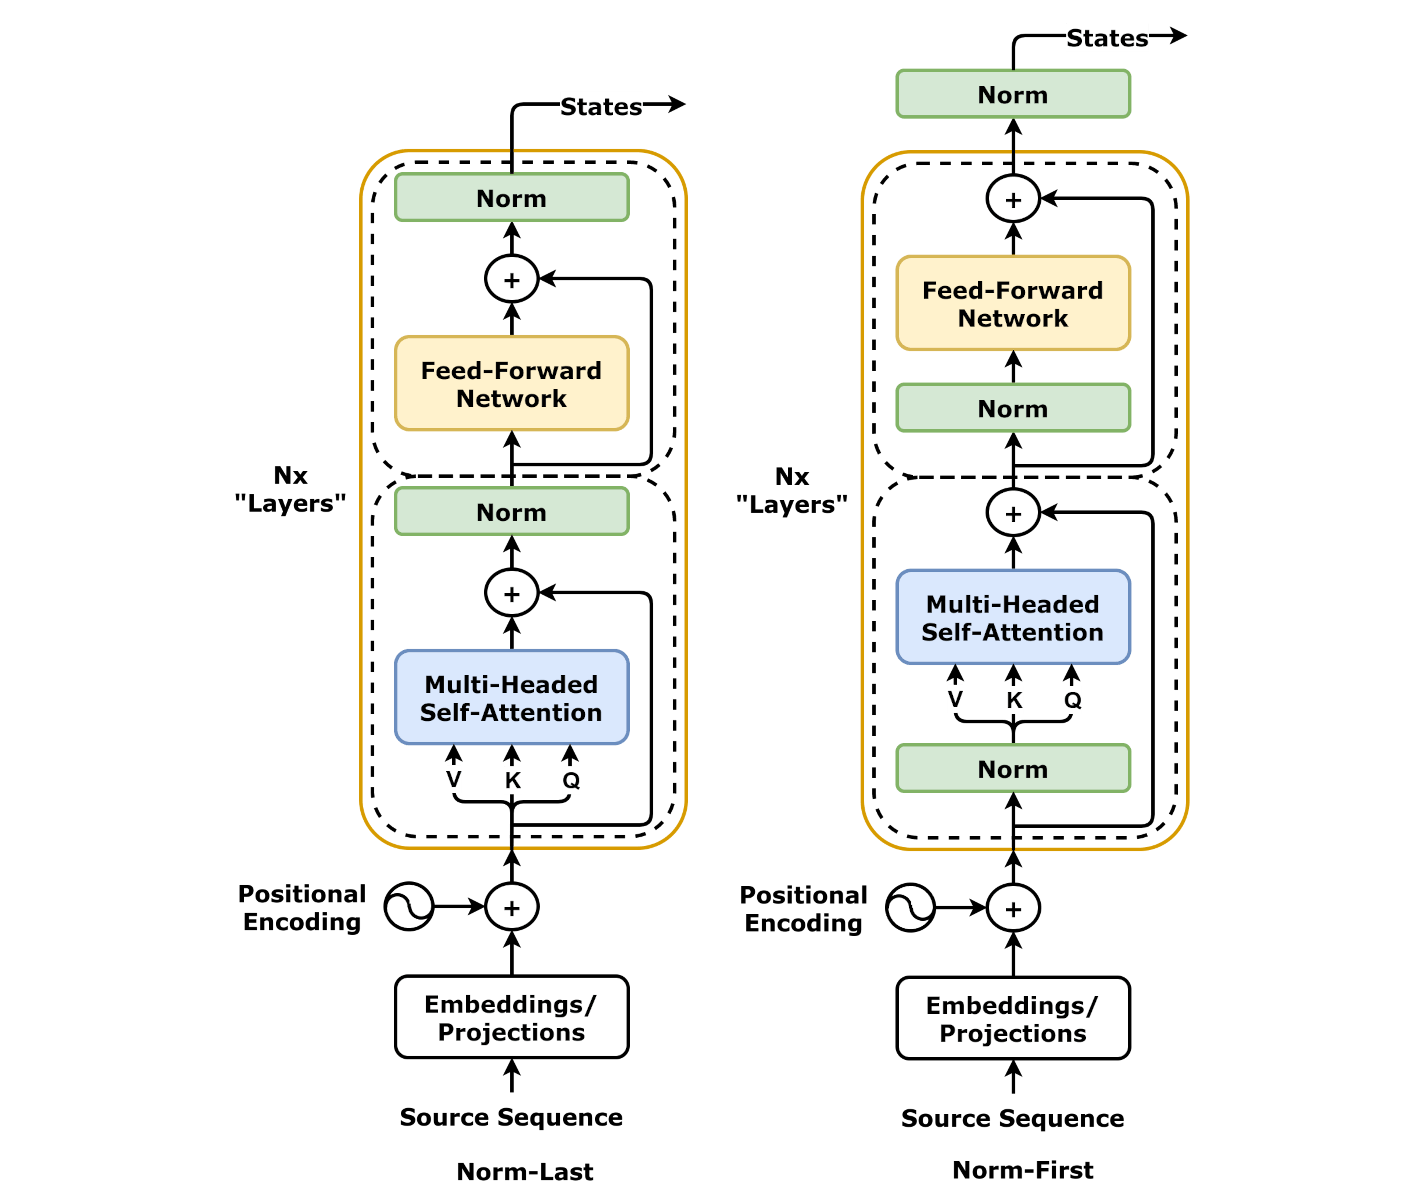
\includegraphics[width=1.5\linewidth]{Images/cap1/Transformer_encoder,_with_norm-first_and_norm-last.png}
        \caption{Differenza tra Encoder Norm Last ed Encoder Norm First}
        \label{fig:encoder}
    \end{minipage}
    \hfill
    \begin{minipage}{0.48\textwidth}
        \centering
		\hspace*{-0.7cm}
        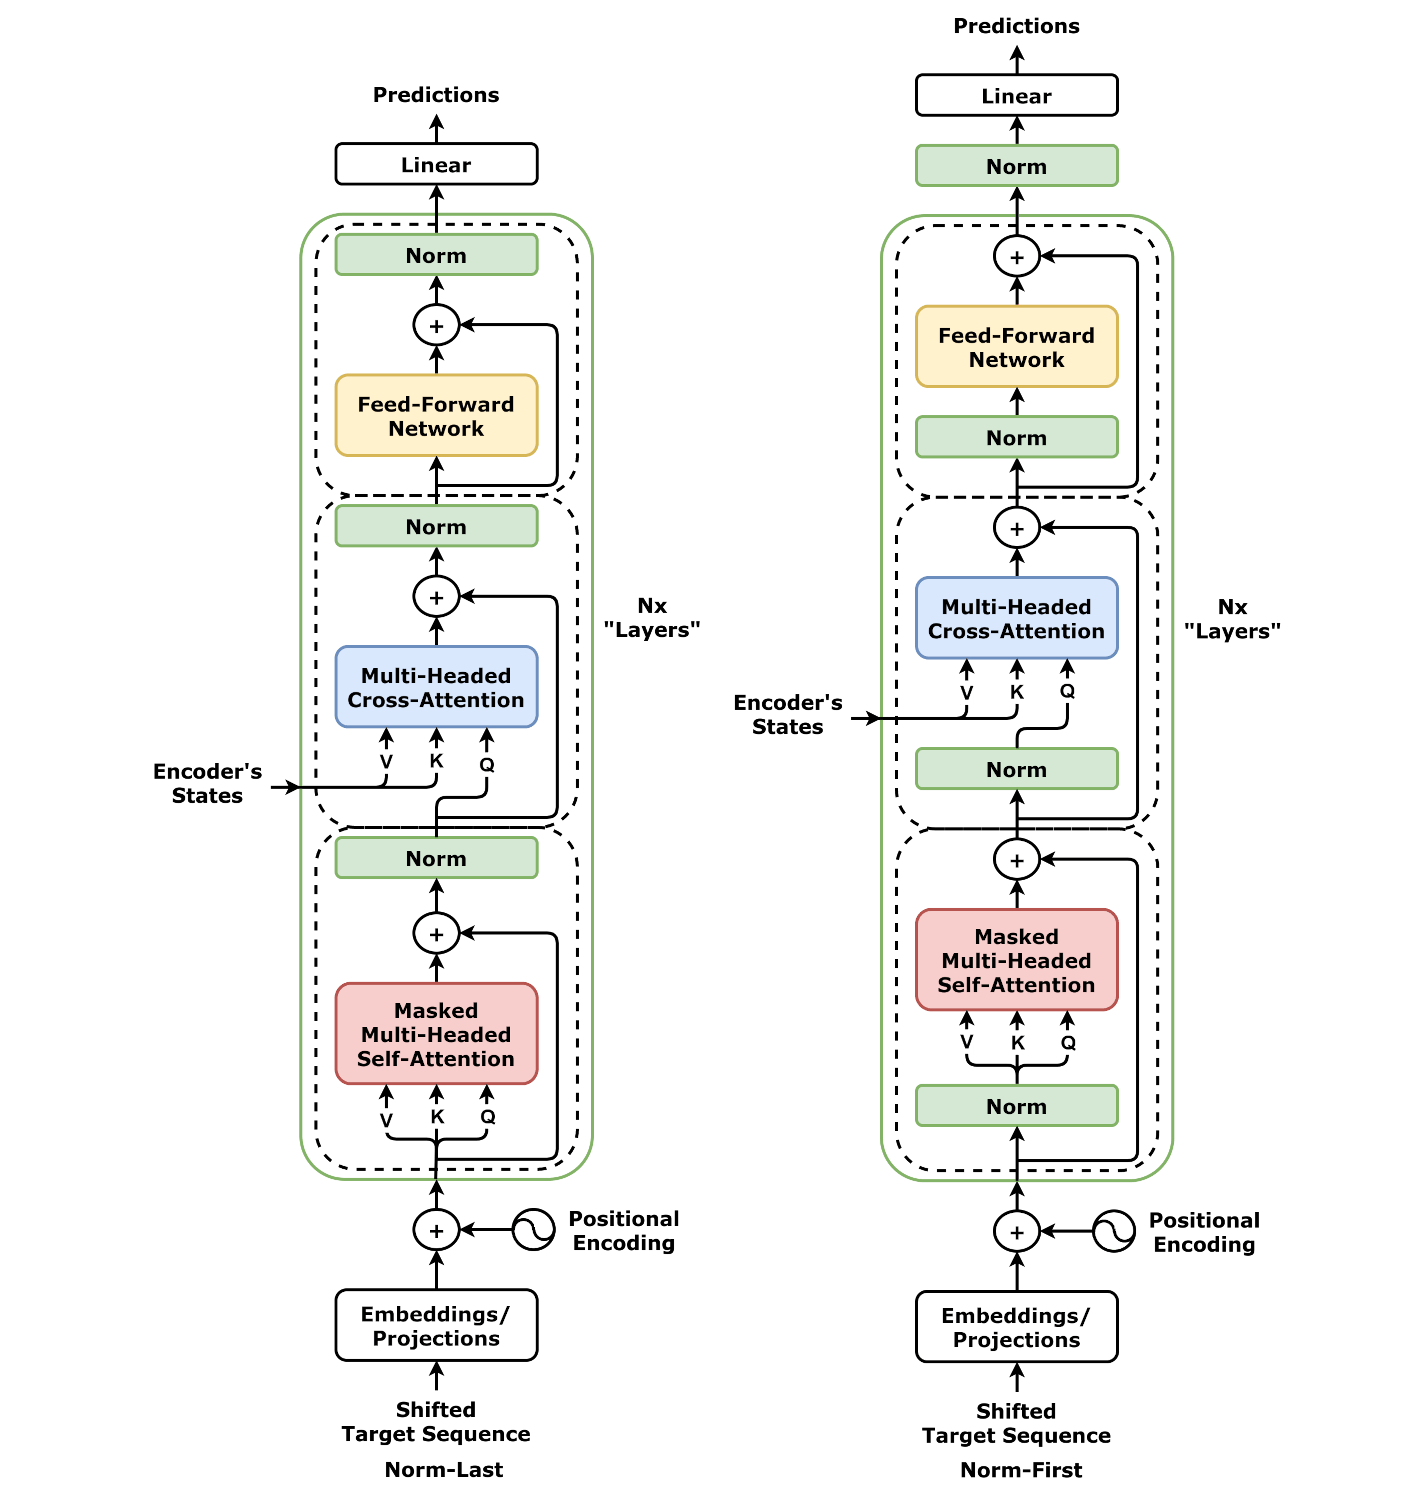
\includegraphics[width=1.2\linewidth]{Images/cap1/Transformer_decoder,_with_norm-first_and_norm-last.png}
        \caption{Differenza tra Decoder Norm Last e Decoder Norm First}
        \label{fig:decoder}
    \end{minipage}
\end{figure}

\subsubsection{Decoder}
Il decoder del Transformer, come l'encoder, è costituito da una pila di \(N\) layer identici (6 in quello originale). Ogni layer del decoder condivide alcune somiglianze con i layer dell'encoder, ma include anche un'importante differenza, data dalla presenza di un terzo sub-layer. Oltre ai due sub-layer che già troviamo nell'encoder, ovvero il Multi-Head Self-Attention Mechanism e la Feed-Forward Neural Network, il decoder introduce un ulteriore sub-layer, chiamato Cross-Attention, che serve a integrare le informazioni elaborate dall'encoder.
I layer del decoder possono essere descritti come segue:
\begin{itemize}
	\item \textbf{Masked Multi-Headed Self-Attention}: Questo sub-layer è simile a quello utilizzato nell'encoder, ma con una differenza fondamentale. Nel decoder, viene applicata una maschera causale (vedi Paragrafo \ref{sec:masked-multi-head-attention}) che impedisce al modello di "guardare" i token futuri. In altre parole, il decoder può prestare attenzione solo ai token già generati e non a quelli successivi, il che è cruciale nei compiti di generazione sequenziale come la traduzione automatica. La maschera causale serve a mantenere la coerenza temporale durante la generazione, garantendo che il modello generi il testo in modo incrementale, senza conoscere in anticipo i token futuri.
	\item \textbf{Multi-Headed Cross-Attention}: Questo secondo sub-layer applica la Multi-Head Attention non solo sui token interni alla sequenza di input del decoder, ma anche sulle rappresentazioni intermedie prodotte dall'encoder. In questo modo, il decoder è in grado di combinare le informazioni che ha già elaborato con le rappresentazioni dell'input elaborate dall'encoder. Questa fase permette al decoder di integrare e "attenzionare" specifiche parti dell'input in base a ciò che ha già generato, creando una connessione tra l'input e l'output che il modello sta costruendo.
	\item \textbf{Feed-Forward Neural Network}: Come nell'encoder, anche qui ogni token è elaborato indipendentemente da una rete neurale feed-forward, che arricchisce le rappresentazioni attraverso trasformazioni non lineari. Questa rete è condivisa in ogni layer e applicata in parallelo su tutti i token della sequenza di output.
\end{itemize}
Tutti e tre i sub-layer sono seguiti da Residual Connections e da un Layer Normalization. Anche in questo caso vale l'osservazione precedente relativa all'ordine di applicazione della normalizzazione nella sequenza di operazioni \cite{xiong2020layernormalizationtransformerarchitecture} (vedi \figurename{~\ref{fig:decoder}}).

\paragraph{Norm-Last vs Norm-First Formula}
L'output generato da ogni sub-layer del Transformer può essere descritto come segue:

Nella versione Norm-Last:
\begin{align}
	\text{Output} = \text{LayerNorm}(x + \text{Sublayer}(x))
\end{align}
Dove \(x\) rappresenta l'input del sub-layer e \(\text{Sublayer}(x)\) la sua elaborazione. La Residual Connection aggiunge l'input originale all'output del sub-layer, mentre il Layer Normalization stabilizza l'addestramento normalizzando le attivazioni.

Oppure nella versione Norm-First:
\begin{align}
	\text{Output} = x + \text{Sublayer}(\text{LayerNorm}(x))
\end{align}

\section{Attention Is All We Need}
Il meccanismo di attenzione è alla base del Transformer ed è fondamentale per gestire le dipendenze tra parole in una sequenza. Può essere descritto come un'operazione di mappatura che prende in input una query e la confronta con un insieme di chiavi (keys) e valori (values), tutti rappresentati da vettori. La query viene confrontata con ogni chiave per calcolare un punteggio di somiglianza, che determina quanto una chiave è rilevante per la query.
Più formalmente, si può dire che l'obiettivo sia calcolare un'uscita pesata dei valori in base alla somiglianza tra la query e le chiavi. Ogni valore viene poi moltiplicato per il punteggio corrispondente, e l'output finale è una somma pesata dei valori.
\begin{itemize}
	\item \textbf{Query}: La query rappresenta l'elemento di input per il quale vogliamo ottenere informazioni rilevanti, in base alle chiavi e ai valori.
	\item \textbf{Keys}: Le chiavi rappresentano gli elementi con cui la query viene confrontata. Ogni chiave ha un valore associato.
	\item \textbf{Values}: I valori sono le informazioni associate a ciascuna chiave, che verranno utilizzate per calcolare l'output.
\end{itemize}
L'output è una somma pesata dei valori, dove i pesi sono dati dalla compatibilità (somiglianza) tra la query e le chiavi, calcolata tipicamente tramite un'operazione come il dot-product (prodotto scalare).
Se necessario (come nel caso del Transformer originale), il prodotto scalare può essere scalato per evitare divergenze nei valori dei pesi causati dall'applicazione della funzione softmax su valori elevati.
\begin{figure}[!t]
	\centering
	\begin{minipage}{0.48\textwidth}
		\centering
		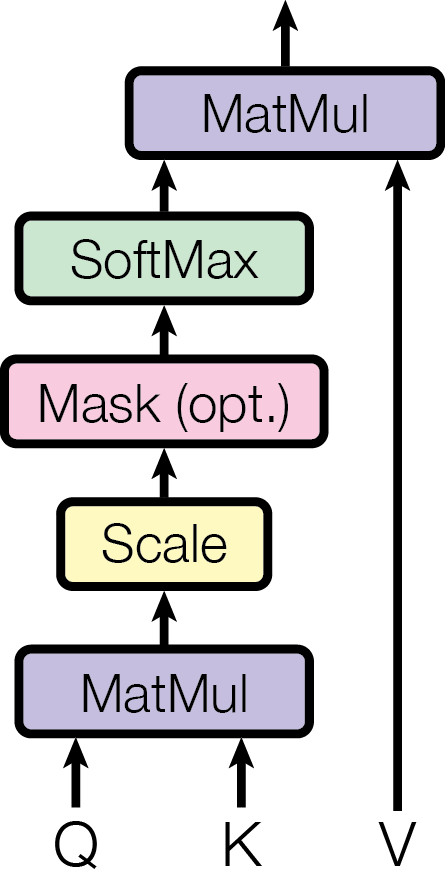
\includegraphics[width=0.5\linewidth]{Images/cap1/ModalNet-19.png}
		\caption{Scaled Dot-Product}
		\label{fig:scaleddotproduct}
	\end{minipage}
	\hfill
	\begin{minipage}{0.48\textwidth}
		\centering
		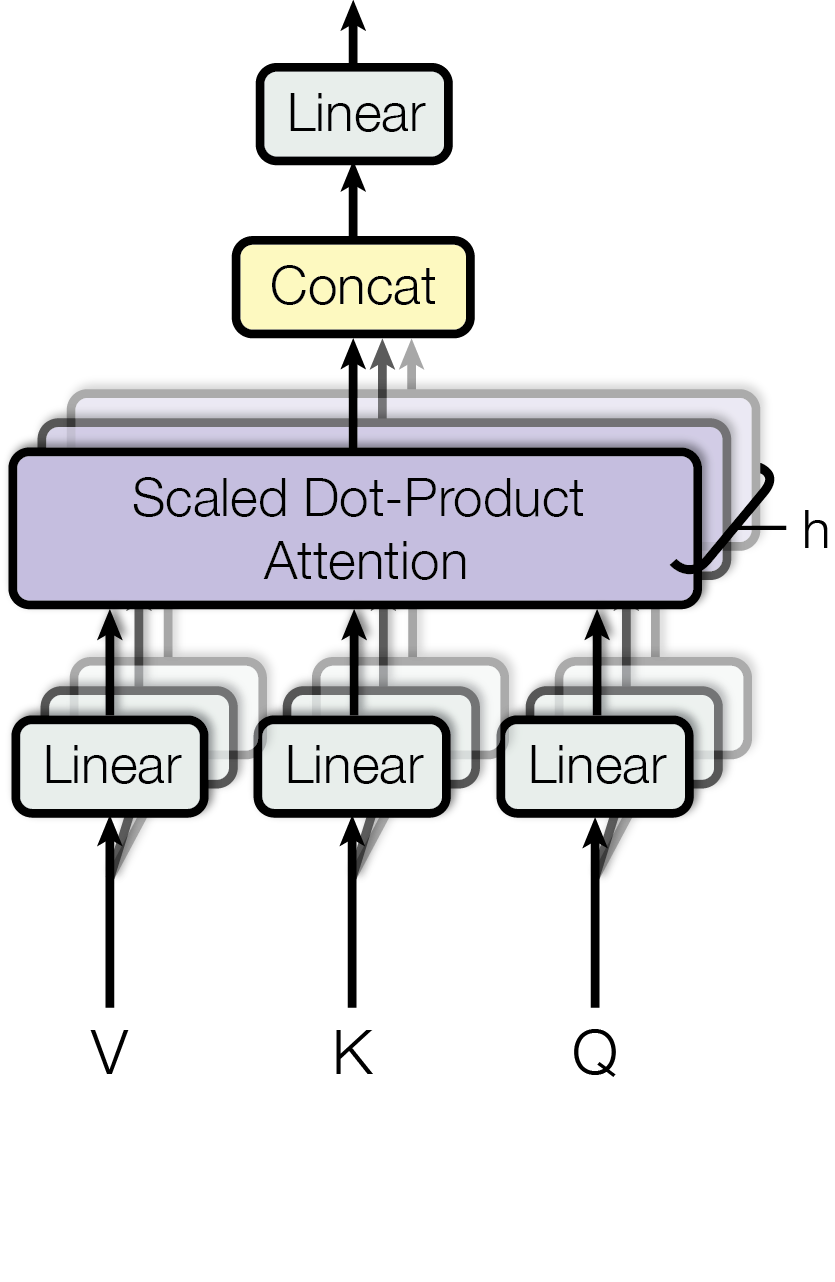
\includegraphics[width=0.65\linewidth]{Images/cap1/ModalNet-20.png}
		\caption{Multi-Head Attention}
		\label{fig:multihead}
	\end{minipage}
\end{figure}
Esistono diverse varianti del meccanismo di attenzione che nel tempo si sono evolute per permettere al modello di diventare più efficiente e, dunque, di avere prestazioni più elevate, come nel caso del Reformer \cite{kitaev2020reformerefficienttransformer} o tramite l'implementazione Flash Attention \cite{dao2022flashattentionfastmemoryefficientexact} che è ottimizzata per calcoli su GPU e TPU in quanto esegue moltiplicazioni tra blocchi di matrici in parallelo. Esiste anche la variante ALiBi (Attention with Linear Biases) \cite{press2022trainshorttestlong} che implementa un meccanismo di positional encoding (vedi Paragrafo \ref{sec:positional-encoding}) aggiuntivo direttamente all'interno del meccanismo di attenzione.

\subsection{Scaled Dot-Product Attention}
Nel paper originale il meccanismo di attenzione viene definito Scaled Dot-Product Attention (vedi \figurename{~\ref{fig:scaleddotproduct}}). L'input dello stesso consiste in un set di vettori query e chiavi di dimensioni \(d_k\), e un set di valori di dimensioni \(d_v\). Vengono calcolati i prodotti scalari di una query con tutte le chiavi e si divide ciascuno di essi per \(\sqrt{d_k}\) (scaling). Infine, si applica una funzione softmax per ottenere i pesi di attenzione sui valori.
Questa procedura viene effettuata su più vettori query parallelamente. Tutti i vettori query vengono inglobati in una matrice \(Q\), i vettori chiave in una matrice \(K\) e i vettori valori in una matrice \(V\). L'output dell'operazione di attenzione è una matrice calcolata con la seguente formula:
\begin{align}
	\text{Attention}(Q, K, V) = \text{softmax}\left(\frac{QK^T}{\sqrt{d_k}}\right)V
\end{align}

\subsection{Multi-Head Attention}
Per catturare relazioni complesse e multidimensionali tra le parole, il Transformer utilizza il meccanismo di Multi-Head Attention (vedi \figurename{~\ref{fig:multihead}}). Questo approccio consente ad esso di apprendere diverse rappresentazioni delle parole attraverso diverse "teste" di attenzione, ciascuna delle quali si concentra su aspetti diversi della sequenza. Ogni testa di attenzione calcola i pesi in modo indipendente, permettendo al modello di cogliere relazioni intricate tra i token e di apprendere rappresentazioni più ricche e dettagliate.

Anziché eseguire una singola operazione di attenzione utilizzando chiavi, valori e query di dimensione \(d_{model}\) (la dimensione dei vettori di embedding), il meccanismo Multi-Head Attention prevede che queste grandezze siano proiettate linearmente \(h\) volte con diverse proiezioni apprese per ottenere chiavi, valori e query di dimensione \(d_k\) e \(d_v\). Su ognuna di queste versioni proiettate di chiavi, valori e query, l'operazione di attenzione viene eseguita in parallelo, producendo come risultato valori in uscita di dimensione \(d_v\).

I risultati delle diverse teste vengono quindi concatenati e proiettati nuovamente per ottenere l'output finale, come mostrato in \figurename{~\ref{fig:multihead}}. Questo processo consente al modello di osservare diversi sottospazi di rappresentazione contemporaneamente, migliorando così la capacità di catturare informazioni da più posizioni nella sequenza \cite{bertattention}. Con un'unica testa di attenzione, infatti, l'operazione media queste informazioni, riducendo la capacità del modello di apprendere relazioni multidimensionali.

Matematicamente, il meccanismo Multi-Head Attention può essere descritto come:
\begin{align}
	\text{MultiHeadedAttention}(Q, K, V) = \text{Concat}(\text{head}_1, \ldots, \text{head}_h)W^O
\end{align}
Dove:
\vspace{-0.25cm}
\begin{align}
	\text{head}_i = \text{Attention}(QW_i^Q, KW_i^K, VW_i^V)
\end{align}
Le proiezioni sono realizzate tramite le matrici dei parametri:
\begin{align}
	W_i^Q \in \mathbb{R}^{d_{model} \times d_k}, \quad W_i^K \in \mathbb{R}^{d_{model} \times d_k}, \quad W_i^V \in \mathbb{R}^{d_{model} \times d_v}, \quad W^O \in \mathbb{R}^{hd_v \times d_{model}}
\end{align}
Nel prototipo originale, sono state utilizzate \(h = 8\) teste di attenzione in parallelo, con \(d_k = d_v = d_{model}/h = 64\). Grazie alla riduzione della dimensione di ciascuna testa, il costo computazionale complessivo rimane simile a quello dell'attenzione a singola testa con la dimensionalità completa.
Il sistema di attenzione multi-testa viene utilizzato in maniera diversa a seconda che si tratti di quello dell'encoder, del decoder o del cross-attention.

\subsubsection{Multi-Headed Self-Attention (Encoder)}
Nell'auto-attenzione nell'encoder, le query, le chiavi e i valori provengono tutti dalla stessa sorgente, ovvero l'output del livello precedente dell'encoder. Ogni posizione nell'encoder può prestare attenzione a tutte le altre posizioni della sequenza elaborata fino a quel punto. Questo consente al modello di catturare relazioni globali tra le parole e costruire rappresentazioni più ricche del contesto testuale. Questo tipo di auto-attenzione è cruciale per comprendere la struttura sintattica e semantica del testo.

\subsubsection{Multi-Headed Cross-Attention (Encoder-Decoder)}
Nell'attività di attenzione encoder-decoder, le query provengono dal livello precedente del decoder, mentre le chiavi e i valori sono generati dall'output dell'encoder. Questo permette a ogni posizione nel decoder di "attenzionare" tutte le posizioni della sequenza di input. In pratica, l'attenzione encoder-decoder consente al decoder di focalizzarsi su specifiche parti della sequenza di input per generare l'output corretto. Questo meccanismo è tipico nei modelli di sequence-to-sequence \cite{sutskever2014sequencesequencelearningneural}, come nei tradizionali modelli di traduzione automatica.

\subsubsection{Masked Multi-Headed Self-Attention (Decoder)}
\label{sec:masked-multi-head-attention}
Anche nel decoder troviamo livelli di auto-attenzione, ma con una particolarità importante: ogni posizione nel decoder può prestare attenzione solo alle posizioni precedenti o uguali della sequenza già generata. Questo comportamento è essenziale per preservare la proprietà auto-regressiva del modello, ovvero l'abilità del decoder di generare il testo in modo sequenziale, senza poter "guardare" il futuro. Per implementare questa restrizione, si applica una maschera che blocca il flusso di informazioni verso destra, mascherando con \(-\infty\)  le connessioni non valide nel calcolo della softmax.

La maschera viene indicata con \(M\) e la funzione di attenzione viene modificata come segue:
\begin{align}
	\text{MaskedAttention}(Q, K, V) = \text{softmax}\left(\frac{QK^T}{\sqrt{d_k}} + M\right)V
\end{align}
Una maschera tipica per il decoder è una matrice triangolare strettamente superiore, che blocca le connessioni tra le posizioni future. Questo garantisce che il modello generi il testo in modo incrementale, senza conoscere in anticipo i token successivi. Questa maschera è chiamata "Maschera Causale" (Causal Mask) e viene applicata a ciascuna testa di attenzione nel decoder.
\begin{align}
	M_{ij} = \begin{cases}
		0 & \text{se } i \leq j \\
		-\infty & \text{altrimenti}
	\end{cases}
\end{align}

\subsection{Position-wise Feed-Forward Networks}
Oltre ai layer attenzionali, sia encoder che decoder sono dotati di un layer di feed-forward neural network, che opera in modo indipendente su ciascuna posizione della sequenza. Questo layer è composto da due layer densi (fully connected) con una funzione di attivazione intermedia, generalmente una ReLU.
\begin{align}
	\text{FFN}(x) = \text{ReLU}(xW_1 + b_1)W_2 + b_2
\end{align}
Solitamente la dimensione dei vettori di embedding viene aumentata nel primo layer e poi ridotta nel secondo, per permettere alla rete di apprendere rappresentazioni più complesse e di ridurre la dimensionalità prima di passare al livello successivo. Questo layer è seguito da un'altra Residual Connection e da un Layer Normalization, per facilitare il flusso del gradiente e stabilizzare l'addestramento.
Sebbene le trasformazioni lineari siano identiche per ogni posizione della sequenza, i parametri utilizzati variano da un livello all'altro. Questo processo può essere descritto come due convoluzioni con kernel di dimensione 1.

\subsection{Positional Encoding}
\label{sec:positional-encoding}
Infine (anche se viene trattato all'inizio della sequenza come parte dell'input, vedi \figurename{~\ref{fig:transformer}}), il Transformer utilizza un meccanismo di codifica posizionale per introdurre informazioni sulla posizione delle parole nella sequenza. Poiché la rete neurale non contiene unità ricorrenti o convoluzionali, che di solito catturano la posizione temporale delle parole, è necessario fornire al modello un modo per distinguere le parole in base alla loro posizione.

Dunque, per risolvere questo problema è possibile aggiungere vettori di posizione (positional encodings) ai vettori di embedding in input. Questi vettori hanno la stessa dimensione dei vettori di embeddings  \(d_{\text{model}}\) così da poter essere sommati direttamente. Per calcolare i vettori di posizione, si utilizzano funzioni trigonometriche \cite{dufter2021positioninformationtransformersoverview}, che permettono di codificare informazioni sulla posizione in modo non lineare. Nel paper originale, vengono utilizzate le seguenti funzioni:
\begin{align}
	\text{PE}_{(pos, 2i)} = \sin\left(\frac{pos}{10000^{2i/d_{\text{model}}}}\right), \quad \text{PE}_{(pos, 2i+1)} = \cos\left(\frac{pos}{10000^{2i/d_{\text{model}}}}\right)
\end{align}
Dove \(pos\) rappresenta la posizione della parola nella sequenza e \(i\) la dimensione del vettore di embedding. In questo modo ogni dimensione del vettore di posizione corrisponde ad una sinusoide e le lunghezze d'onda variano in base alla posizione formando una progressione geometrica che va da \(2\pi\) a \(10000 \cdot 2\pi\). Questa funzione è stata scelta poiché si ipotizzava che avrebbe facilitato il modello nell'apprendimento delle posizioni relative poiché per ogni offset costante \(k\), \(\text{PE}_{(pos + k)}\) può essere rappresentato come una funzione lineare di \(\text{PE}_{(pos)}\).

Esistono varianti che utilizzano approcci convoluzionali \cite{gehring2017convolutionalsequencesequencelearning} che hanno dato risultati simili, ma si preferisce usare funzioni sinusoidali perché si ritiene che consentano al modello di generalizzare meglio su sequenze di lunghezza superiore rispetto a quelle incontrate durante l'addestramento. Successivamente si è scoperto che anche senza applicare la codifica posizionale, si è in grado di apprendere informazioni posizionali grazie all'applicazione della maschera causale nel decoder \cite{haviv2022transformerlanguagemodelspositional}.
Successivamente sono stati sviluppati algoritmi di Relative Positional Encoding \cite{shaw2018selfattentionrelativepositionrepresentations} che permettono la codifica delle posizioni relative tra le parole, migliorando la capacità del Transformer di catturare relazioni spaziali tra le parole. Questo approccio è differente da quello originale, che codifica solo la posizione assoluta delle parole \cite{ke2021rethinkingpositionalencodinglanguage}.